\documentclass{cmspaper}
\usepackage{epsf}
\usepackage{epsfig}
\begin{document}

%==============================================================================
% title page for few authors

\begin{titlepage}

% select one of the following and type in the proper number:
   \cmsnote{2008/000}
%  \internalnote{2005/000}
%  \conferencereport{2005/000}
   \date{23 July 2008}

  \title{Photon Identification for CMS Startup}

  \begin{Authlist}
    A.~Askew, O.~Atramentov, Y.~Gershtein,
       \Instfoot{FSU}{Florida State University, Tallahassee, FL.}

    A.~Debenedetti,
	\Instfoot{Minn}{University of Minnesota, Minneapolis, MN.}

    M.~Gataullin, V.~Litvin, J.~Veverka, 
	\Instfoot{CalTech}{California Institute of Technology, Pasadena, CA.}

    C.~Kopecky, T.~Miceli, J.~Stilley, M.~Tripathi
	\Instfoot{UCDavis}{University of California at Davis, Davis, CA.}

    V.~Gaultney,
        \Instfoot{FIU}{Florida International University, Miami, FL.}

    S.~Shrestha,
        \Instfoot{KSU}{Kansas State University, Manhattan, KS.}

    M.~Anderson,
        \Instfoot{Wisc}{University of Wisconsin, Madison, WI.}

    J.~Lamb
        \Instfoot{UCSB}{University of California at Santa Barbara, Santa Barbara, CA.}

    M.~Mozer
	\Instfoot{IIHE}{IIHE, Brussels, Belguim.}

    N.~Marinelli
        \Instfoot{ND}{University of Notre Dame, Notre Dame, IN}

  \end{Authlist}

% if needed, use the following:
%\collaboration{Flying Saucers Investigation Group}
%\collaboration{CMS collaboration}

  \begin{abstract}
This note defines the methods by which the identification of photons may be verified from data
on start up.  This verification includes measurement of the photon efficiency, as well as methods
for obtaining photon purity.  Backgrounds to photons from jets and electrons are discussed, and an
example set of ``vanilla'' photon identification requirements are presented. 
  \end{abstract} 

% if needed, use the following:
%\conference{Presented at {\it Physics Rumours}, Coconut Island, April 1, 2005}
%\submitted{Submitted to {\it Physics Rumours}}
%\note{Preliminary version}
  
\end{titlepage}
\tableofcontents
\listoffigures
\listoftables
\pagebreak

\setcounter{page}{2}%JPP

\section{Introduction}
Photon identification at hadron colliders is a difficult task, mainly due to the large backgrounds from hadronic jets and
the lack of a clean large cross-section resonance decaying into high $E_T$ photons for studies.  
Radiative decays $Z\gamma\rightarrow\ell\ell\gamma$ events in which the photon is radiated off one of the final state leptons 
can be selected and used for photon calibration \cite{uug_note}, but the rate of this decay is small and photons tend to be soft.
This difficulty is further compounded by the fact that unlike electrons,
photons are not redundant
\footnote{Unconverted photons are not redundant.  For the special case of conversions with reconstructed
tracks, please see~\cite{NancyConv}.}, e.g. they leave a signal in only one detector, the electromagnetic calorimeter.  
Thus, unlike electrons, tracker and calorimeter information can not be compared to get a handle on the reconstruction efficiency.
Also, photons are subject to backgrounds (such as cosmic/halo muon bremsstrahlung) which do not typically afflict electrons.
Special techniques are being developed to measure and reduce these non-collision backgrounds.

This note describes a possible strategy for doing physics with photons at very early stages of the experiment.
CMS detector combines very heavy tracker with very strong magnetic field. The effects of both on electrons and photons are very significant, and are 
unlikely to be well-described by the Monte Carlo simulation in the beginning of the run. 
We show that a moderately effective photon identification can be constructed so that its efficiency and purity can be reliably measured with
data itself.

We show that some identification variables, like hollow cone track isolation and cluster width in $\eta$, are quite similar between electrons and 
photons and therefore can be calibrated using $Z \rightarrow e e$ decays. 
These efficiencies can then be (to the limit of available statistics) verified with early samples of $Z\gamma\rightarrow\ell\ell\gamma$.  
We also show that selecting photon candidates failing hollow cone track isolation in multi-jet events 
provides us with a clean sample of pure and minimally biased jet background for fake rate determination.


\section{Photon Reconstruction and LooseEM}

In order to utilize the flexibility of the photon reconstruction software, a base definition {\bf LooseEM} 
is defined to provide a starting point for both signal and background studies\footnote{There is a software 
delineation between the EgammaPhotonProducer package, which constructs the actual reco::Photon, and the 
PhotonIdentification package which is mainly concerned with the organization and analysis of reco::Photon 
objects.  The interested reader is referred to Appendix B.}.  The object of the {\bf LooseEM} definition is 
to provide a definition of objects that are reconstructed as photons which are 100\% efficient for true photons 
(produced in collisions), but provides some rejection against fake photons from hadronic activity. In particular, 
it ensures that a jet gives rise to not more than one of such objects, and that its energy is comparable to 
the parent parton. 

A {\bf LooseEM} for the purposes of this documents is defined as a reco::Photon which meets the following criteria:
\begin{list}{$\bullet$}
 \item{The reco::Photon must be isolated from other deposits of energy in the ECAL.  The sum of the energy deposited in a cone
of $\Delta R <$0.4 minus the energy that is clustered into the photon must be smaller than 20~GeV.  The distribution of the sum is presented in 
Figure~\ref{fig:EMiso_EMLoose}. All crystals with $E_{crys} >$ 0 GeV are considered. Higher thresholds are likely to improve the discrimination
and are being optimized (also in context of electron and muon isolation).}
 \item{The reco::Photon must be isolated from surrounding deposits of energy in the HCAL.  The sum of the energy in the HCAL in
a hollow cone of 0.1 $< \Delta R<$0.4 is required to be smaller than 10~GeV.  No threshold save that the cells are above 0 GeV is applied.  
Note that the selection of this hollow cone is to make the measurement of this isolation quantity independent of the calculation of the 
hadronic-electromagnetic energy ratio which is more sensitive to EM shower leakage.}
 \item{The reco::Photon is required to have its $HadOverEM$ ratio be smaller than 0.2.  $HadOverEM$ here is defined as the energy within $\Delta R=$0.1 of the supercluster centroid in the hadronic calorimeter divided by the energy of the supercluster.}  
\end{list}

Distributions of each of these quantities are shown for nominal samples of signal and background in Figures~\ref{fig:EMiso_EMLoose},~\ref{fig:HCALiso_EMLoose}, and~\ref{fig:HadOverEM_EMLoose}.  All of these distributions are shown for barrel photons only.

\begin{figure}[hbtp]
  \begin{center}
    \resizebox{10cm}{10cm}{\includegraphics{EMLoose/EMiso_EMLoose.eps}}
    \caption{ECAL isolation energy for direct photons (blue) and for fakes from dijets (red).}
    \label{fig:EMiso_EMLoose}
  \end{center}
\end{figure}
\begin{figure}[hbtp]
  \begin{center}
    \resizebox{10cm}{10cm}{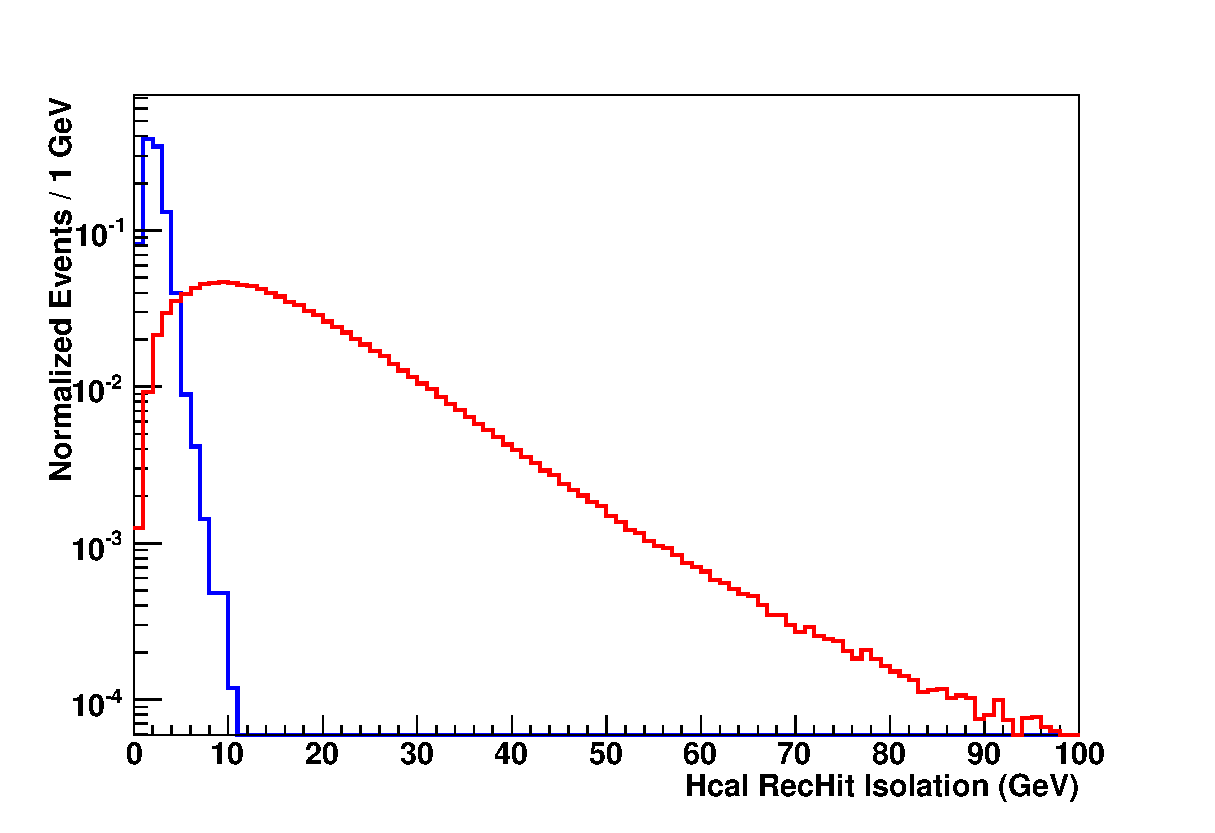
\includegraphics{EMLoose/HCALiso_EMLoose.eps}}
    \caption{HCAL isolation energy for direct photons (blue) and for fakes from dijets (red).}
    \label{fig:HCALiso_EMLoose}
  \end{center}
\end{figure}
\begin{figure}[hbtp]
  \begin{center}
    \resizebox{10cm}{10cm}{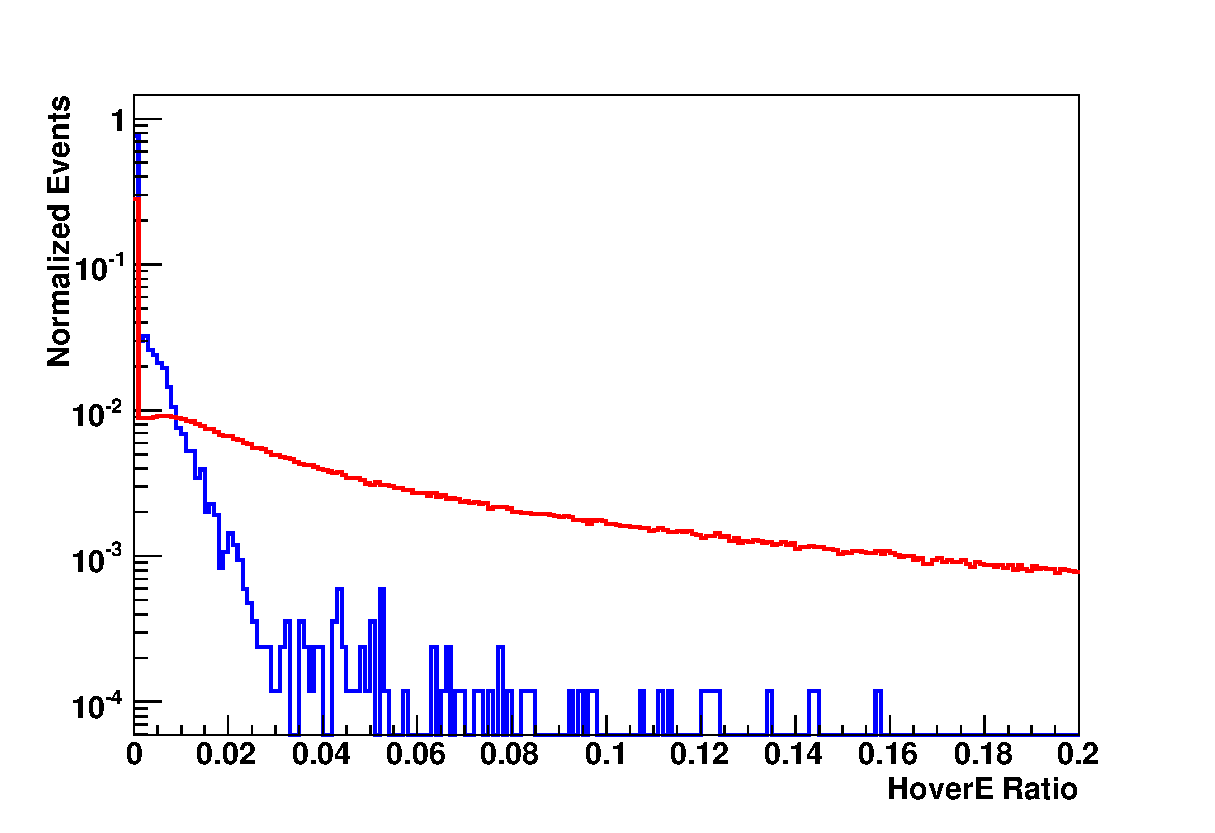
\includegraphics{EMLoose/HadOverEM_EMLoose.eps}}
    \caption{HadOverEM ratio for direct photons (blue) and for fakes from dijets (red).  No photon overflows are present.}
    \label{fig:HadOverEM_EMLoose}
  \end{center}
\end{figure}

The signal sample shown here is a sample of QCD direct photon production (explicitly generated in the 40-60~GeV range) produced privately 
in CMSSW\_2\_1\_0\_pre5, in which the generated photon was required to match to a reconstructed reco::Photon object.  The background sample 
was a sample of inclusive QCD dijets which were produced in the official CSA08 production, which made use of CMSSW\_2\_0\_5.  As previously 
mentioned, only barrel photons are considered here, and further, the photon $E_{T}$ is required to be greater than 20~GeV.
As one can see, these cuts remove a significant portion of the jet background, while retaining most if not all of the true photons.  
The efficiency of these cuts, and their measurement from the data is discussed in Section~\ref{ssec:LooseEMEff}.

\section{Photon Identification Quantities and Selection}
With the base {\bf LooseEM} definition in place, more specific selection cuts for photon identification may be chosen.  Two additional 
definitions are made here {\bf LoosePhoton} and {\bf TightPhoton}.  
A {\bf LoosePhoton} is defined as a {\bf LooseEM} with:
\begin{list}{$\bullet$}
 \item{$HadOverEM$ ratio of smaller than 0.1.}
\item{Isolation from electromagnetic activity (as defined in {\bf LooseEM}) smaller than 15 GeV.}
\item{The sum of the $p_{T}$ of tracks within a hollow cone of $\Delta R<$(0.4-0.04) is required to be smaller than 5 GeV.  Only tracks which are
within 2~cm of the reconstructed vertex z-position are considered for this sum.}
\end{list}
A {\bf TightPhoton} satisfies all of the cuts from the {\bf LoosePhoton}, but with the additional requirement that its R9 variable (defined in Eqn.~\ref{eqn:R9}) is greater than 0.8.
\begin{equation}
 R9 = \frac{E_{3x3}}{E_{supercluster}}
\end{equation}\label{eqn:R9}
\begin{figure}[hbtp]
  \begin{center}
    \resizebox{10cm}{10cm}{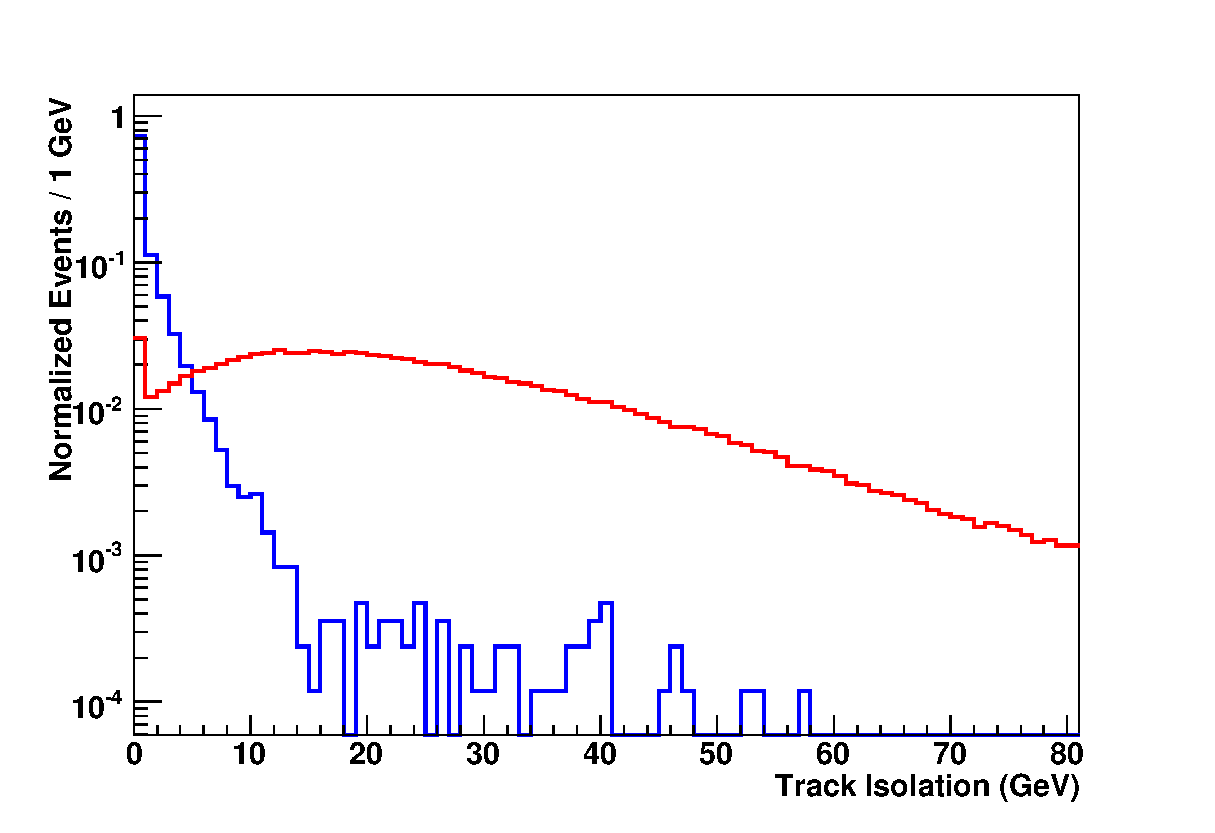
\includegraphics{PhotonSel/Photonid_trkiso.eps}}
    \caption{Sum of track $p_T$ as defined in {\bf LoosePhoton} for {\bf LooseEM} objects in direct photon events (blue) and fakes
from dijets(red).}
    \label{fig:Photonid_trkiso}
  \end{center}
\end{figure}
\begin{figure}[hbtp]
  \begin{center}
    \resizebox{10cm}{10cm}{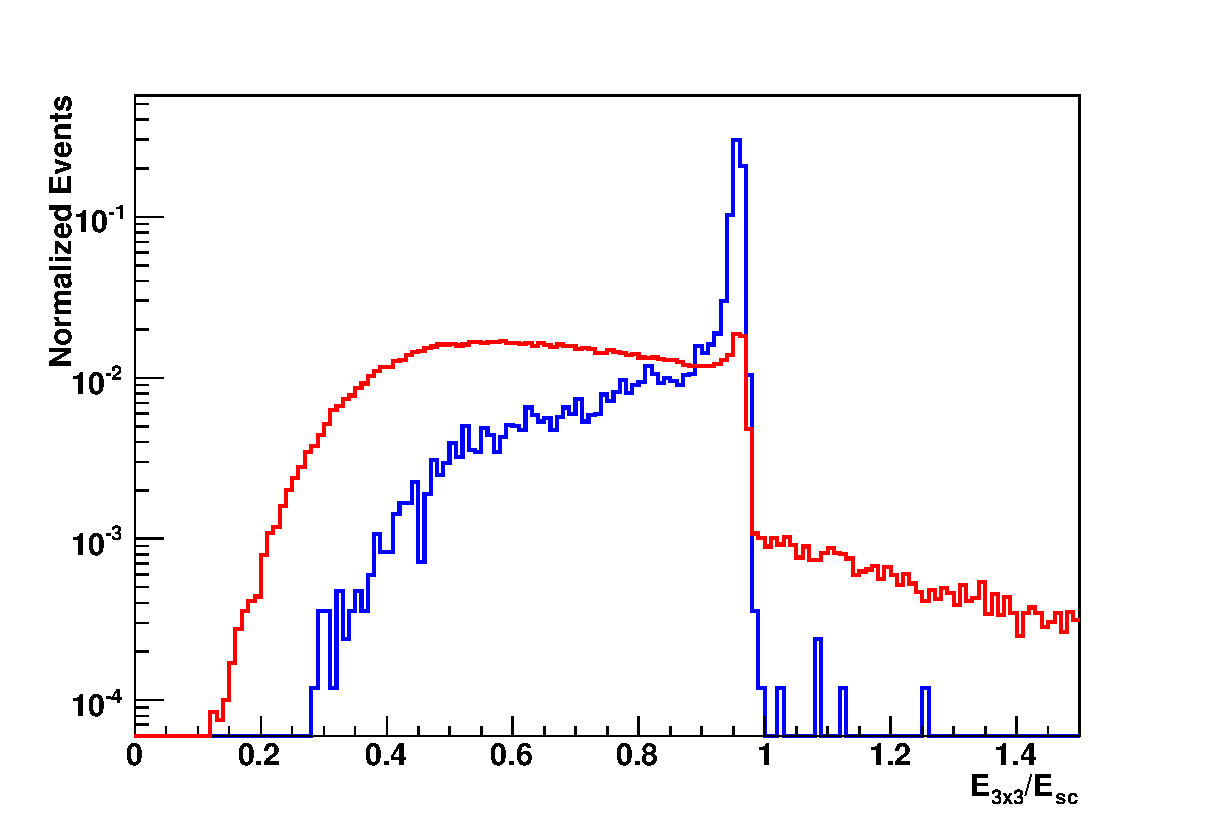
\includegraphics{PhotonSel/Photonid_r9.eps}}
    \caption{R9 variable for {\bf LooseEM} objects in direct photon events (blue) and for fakes from dijets (red).}
    \label{fig:Photonid_r9}
  \end{center}
\end{figure}

\section{Efficiency Determination in the Data}
Since photons are not redundant objects (as previously stated), the determination of the data efficiency for photon reconstruction requires more steps than the simple tag-and-probe method for electrons from $Z\rightarrow ee$ events.
The base prescription for measuring photon efficiencies in data shall be:
\begin{list}{$\bullet$}
\item{Make selection on quantities that will be as similar as possible between electrons and photons.  A good example of this is the hollow cone of the track isolation, which will be set such that for electrons the associated track will be outside this
cone such that the track isolation efficiency can be measured with electrons.}
\item{Ascertain the extent to which a cut can be made on these similar quantities.  If a cut on, say track isolation, is noticeably different between electrons and photons in the Monte Carlo, then this difference must be assigned as a systematic uncertainty.}
\item{Measure the efficiency for the given selection cuts in data using a tag-and-probe method.  Use this same tag-and-probe method to measure the efficiency in Monte Carlo, and compare with the Monte Carlo truth efficiency to check for bias.} 
\item{Scale the Monte Carlo efficiency (if necessary) to the data and calculate the final systematic uncertainty.}
\end{list}

This prescription limits one, for early data taking, to quantities that can be verified in the data from electrons.  Of course, constructing quantities that are similar for photons and electrons allows one to factorize the background somewhat, first there will be hadronic jets (which are discriminated against by the different isolation requirements), and isolated electromagnetic objects.  These electromagnetic objects, by means of a track veto, can then be separated into electrons and photons. 
\subsection{LooseEM efficiency}\label{ssec:LooseEMEff}

It is very difficult to measure the clustering efficiency of an unconverted photon. For this, we must rely on Monte Carlo.
However, the Monte Carlo can be cross-checked using electrons, and if the measured efficiency is large then the resulting systematic 
error can be made small. 

The {\bf LooseEM} efficiency for electrons is determined using a tag-and-probe method.  $Z$-boson events are selected first by requiring two 
high $p_T$ tracks, one of which is required to match well (in $\eta-\phi$) with an electromagnetic object in the ECAL.  The second serves as a probe, 
and along with the cluster matched to the tag, the invariant mass can be formed, to control possible backgrounds.  The efficiency then, is the 
rate at which the probe track is associated with a {\bf LooseEM} object in the calorimeter.

\subsection{Photon Efficiencies}

\subsubsection{Track Isolation Inner Cone}
As previously mentioned, the track isolation cut is meant to be efficient for both electrons and photons.  The goal of this requirement is to separate
electromagnetic objects such as electrons and photons from hadronic fakes (from dijets).  Thus the inner cone of the track isolation hollow cone must be set such that it does not include the tracks from electrons, and ideally, gives a similar efficiency for electrons and photons.  
In the Monte Carlo, a study was performed to determine the width of this inner cone.  A sample of $Z\rightarrow ee$ events, from the CSA08 start up scenario
Monte Carlo was used, along with the previously mentioned direct photon Monte Carlo.  A tag and probe method was used on the $Z$ events, requiring two barrel {\bf LooseEM} objects, with $E_T$ greater than 20~GeV.  One of these objects, the tag, was required to match spatially well to a high $p_T$ track (greater than 10~GeV), while the track isolation was calculated for the other object.  The events passing and failing this tag-and-probe method in the invariant
mass range from 80-100~GeV were then summed up and the efficiency calculated.  This efficiency was then compared to the Monte Carlo truth efficiency for
the electrons, with no tag-probe requirements (associating the Monte Carlo electron to a reconstructed {\bf LooseEM} object and subsequently calcuating the track isolation).  Then these curves were compared with the truth efficiency for photon objects (similar to the truth efficiency for the electrons).  These efficiencies are shown in Figure~\ref{fig:innerConeScan}.  As one can see, the probability for the track from the electron to fall outside of the inner cone
is minimized at $\Delta R >$0.04.  These efficiencies are also in good agreement with the efficiency of the photon at this point as well.

\begin{figure}[hbtp]
  \begin{center}
    \resizebox{10cm}{10cm}{\includegraphics{PhotonSel/CompareFinalTrkInnerCone.eps}}
    \caption{Efficiency of requiring that the sum of track $p_T$ in a hollow cone is smaller than 5~GeV as a function of the inner cone radius.  The efficiency of the tag-and-probe method on Monte Carlo electrons is shown in red.  The efficiency of the Monte Carlo truth electrons is shown in black.  The Monte
Carlo truth efficiency for photons is shown in green.}
    \label{fig:innerConeScan}
  \end{center}
\end{figure}

\subsection{Photon ID with \boldmath $\mathrm{Z}\to \ell^+\ell^- \gamma$ Events}
As described in the previous section, the
performance of photon identification cuts  can be  studied with $\mathrm{Z} \to\mathrm{e}^+\mathrm{e}^-$
decays. However, the majority of electrons lose a significant amount of energy in the tracker via bremsstrahlung while curving 
in the strong magnetic field of CMS. On contrary, a large fraction of central photons will not convert until reaching
the ECAL. In addition, the effects of photon conversions cannot be reliably studied
with electrons. Therefore, it is preferable to cross-check the results of such studies with a photon-enriched sample.
At LHC, the center-of-mass energy and luminosity are high enough to provide a source of clean isolated photons
 from radiative Z decays  $\mathrm{Z}\to \ell^+\ell^- \gamma$, $\ell =\mathrm{e},\mu$. 
In this section, we describe the event selection in the presence of significant
hadronic backgrounds and give  estimates of the expected photon yields.


To obtain predictions for the  $\mathrm{Z}\to \ell^+\ell^- \gamma$ signal (FSR) and backgrounds from initial-state
radiation and $\mathrm{Z}+jets$, the  inclusive
PYTHIA $\mathrm{pp} \to (\mathrm{Z^*}/\gamma^*) \to \ell^+\ell^-$ samples are used. Here the FSR signal is isolated
by using the generator-level matching.
The inclusive $\mathrm{pp} \to t\bar{t}$  background was produced with TOPREX. To estimate
the   $\mathrm{pp} \to b\bar{b}$ we used both the ``official'' ppllX sample, as well as a privately produced
sample of $ b\bar{b} \to \ell^+\ell^- +X$ events. The above MC samples for the $ \mu^+\mu^- \gamma$ final
state are detailed in Table~\ref{tab:lgamma}.

\newcommand{\bbmmX}{\ensuremath{b\bar{b}\rightarrow \mu^+\mu^-X}}
\newcommand{\ttbar}{\ensuremath{t\bar{t}}}

  \begin{table}[htb]
    \caption{Monte Carlo data samples used in this study.}
%    \label{tab:mcsamples}
    \begin{center}
      \begin{tabular}{|l|r|r|r|l|} \hline
                 & \multicolumn{1}{l|}{Events per $100 pb^{-1}$}
                          &                &          &
                             \\
        Process     & \multicolumn{1}{l|}{after selection}
                          & $N_\mathrm{evt}$
                                & \multicolumn{1}{c|}{$\sigma$}
                                           & DBS
                             \\
      \hline\hline
        incl. Z  & 571 (FSR) + 44 (bkgd.)
                          &  1M & 835 pb   &
/Zmumu/CMSSW\_1\_6\_7-CSA07-1192835913                 \\
        \ttbar   & 16     &  1M & 850 pb   &
/ttbar\_inclusive\_TopRex/CMSSW\_1\_3\_1-Spring07-1122 \\
        \bbmmX   & 14     &  1M & 7.52 nb  & private production with
CMSSW\_1\_6\_7                 \\
        $pp\rightarrow l^+l^-X$
                 &        &  2M & 335 nb   &
/ppllX/CMSSW\_1\_6\_7-CSA07-1201845688/RECO            \\
      \hline
      \end{tabular}
    \end{center}
  \end{table} \label{tab:lgamma}


We require that the leading lepton candidate should have $E_T > 15$~GeV, and the trailing lepton  $E_T > 10$~GeV.
The photon candidate is required to be in the barrel region and have  $E_T > 10$~GeV.
We then apply kinematic cuts to improve the signal-to-background ratio. 
Signal photons are radiated from leptons so that their direction should be close to the direction of 
one of the leptons in the event. We require that the $\Delta R$ distance between the closest lepton and photon
should be less than 0.9 (see Figure~\ref{fig:llgamma}a). 
Since one of the main backgrounds is Drell-Yan, it can be suppressed with a cut on the $\ell^+\ell^-$ invariant mass 
$45 < M_{\ell\ell} < 85$~GeV, as shown in Figure~\ref{fig:llgamma}b). The  $t\bar{t}$ events are expected to have
a significant jet activity in the detector. To suppress such events, we apply a simple jet-veto by
requiring that the $E_T$ of the second leading central jet that is not matched to the photon 
 ($\Delta R > 0.4$) should be below 15~GeV 
(see Figure~\ref{fig:llgamma}c). Furthermore, to suppress the $b\bar{b}$ background we apply stringent
ECAL, HCAL, and and track isolation cuts on the lepton furthest away from the photon. No 
isolation requirements on the
photon candidate or the lepton closest to it are applied, which should make the future studies of the photon ID cuts
virtually unbiased. Finally, we require that the three-body $\ell^+\ell^-\gamma$ invariant mass should
be close to the Z mass: $ 85 < M_{\ell\ell\gamma} < 97$~GeV.

As shown in Figure~\ref{fig:llgamma}d), the $E_T$  spectrum of the photon candidates is quite soft, however
an almost complete suppression of the background is possible for the  $\mu^+\mu^-\gamma$ final state.
The expected event yield is expected to be about 650 events per 100~pb$^{-1}$, with a sample purity of 89\%.
Increasing the photon $E_T$ cut to $E_T > 20$~GeV, will reduce the signal sample by 70\%. The expected
event rates for the signal and considered backgrounds are detailed in Table~\ref{tab:lgamma}.

Due to possible overlap of the electron and photon showers, a similar  selection of 
the $\mathrm{e}^+\mathrm{e}^-\gamma$
events is less efficient. The total event yield is found to be about 320~events per 100~pb$^{-1}$, 
with a sample purity of 74\%. The obtained three-body invariant mass spectra are compared 
in Figures~\ref{fig:llgamma}e,f). For both final states, the  $\ell^+\ell^-\gamma$ peak width 
is found to be about 4\%.


\begin{figure}[p]
  \begin{center}
    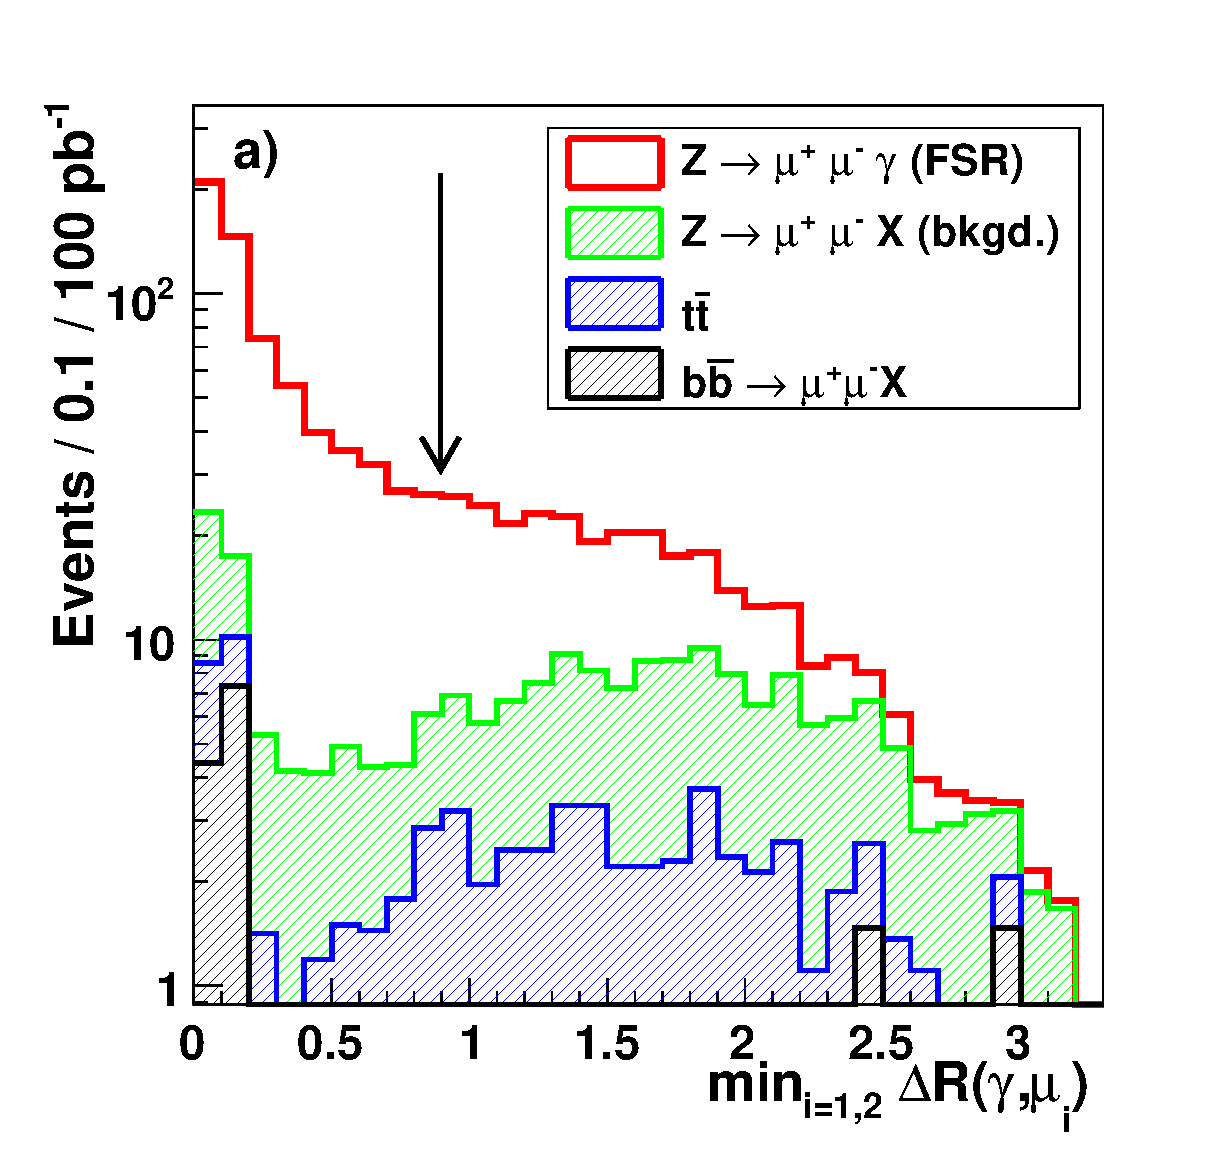
\includegraphics[width=0.46\linewidth]{zgammafigs/drMinGM.eps}
    \includegraphics[width=0.46\linewidth]{zgammafigs/drmMM.eps} %%\\[2mm]
    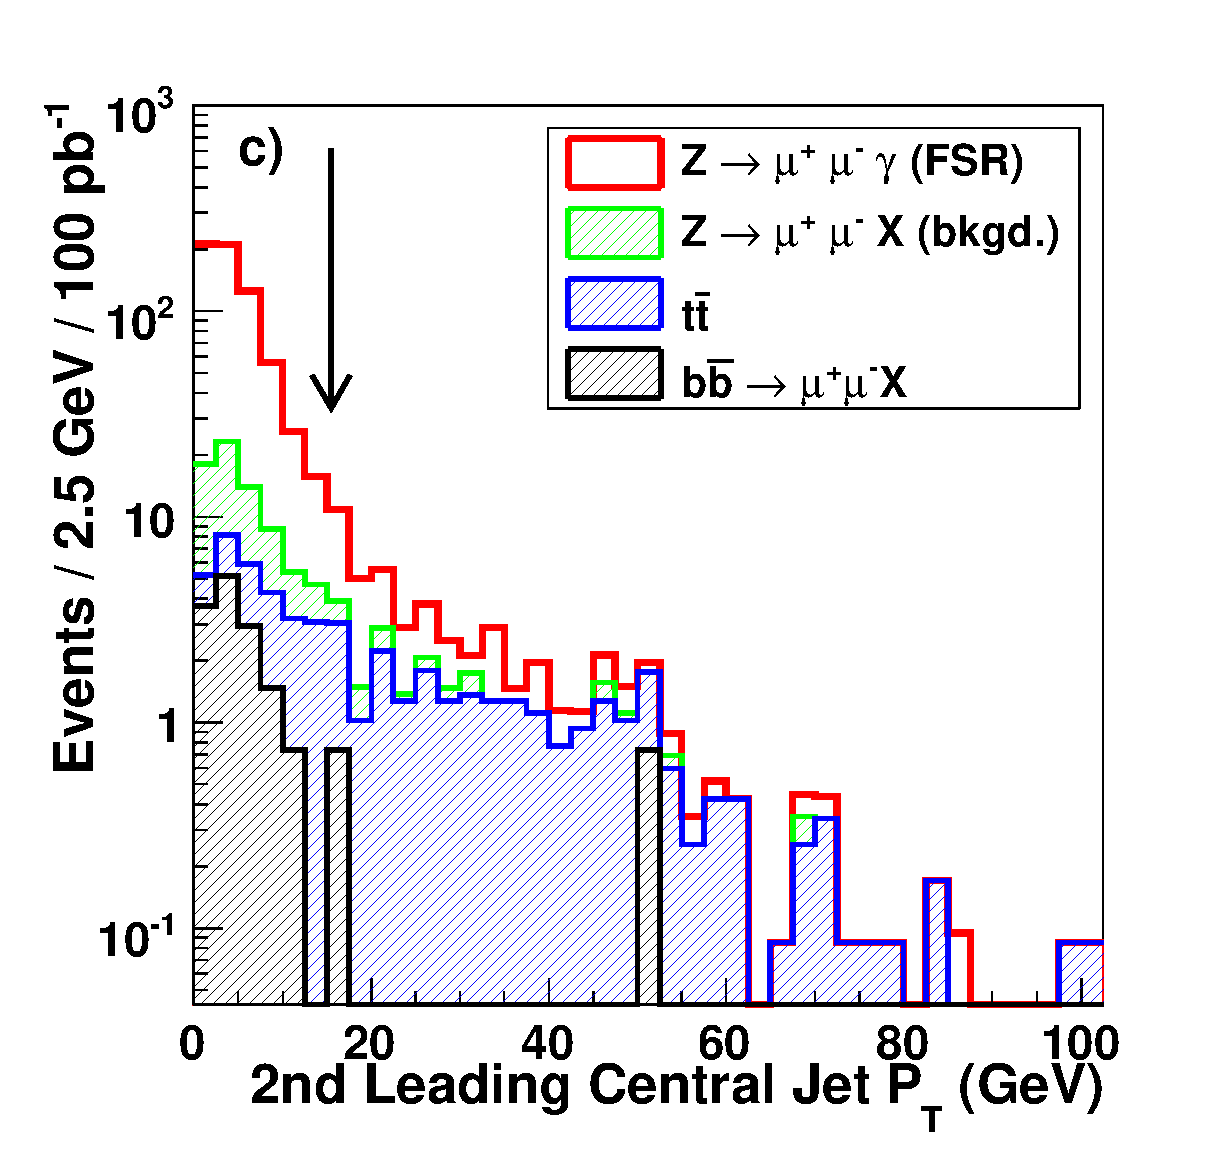
\includegraphics[width=0.46\linewidth]{zgammafigs/ptJL2.eps}
    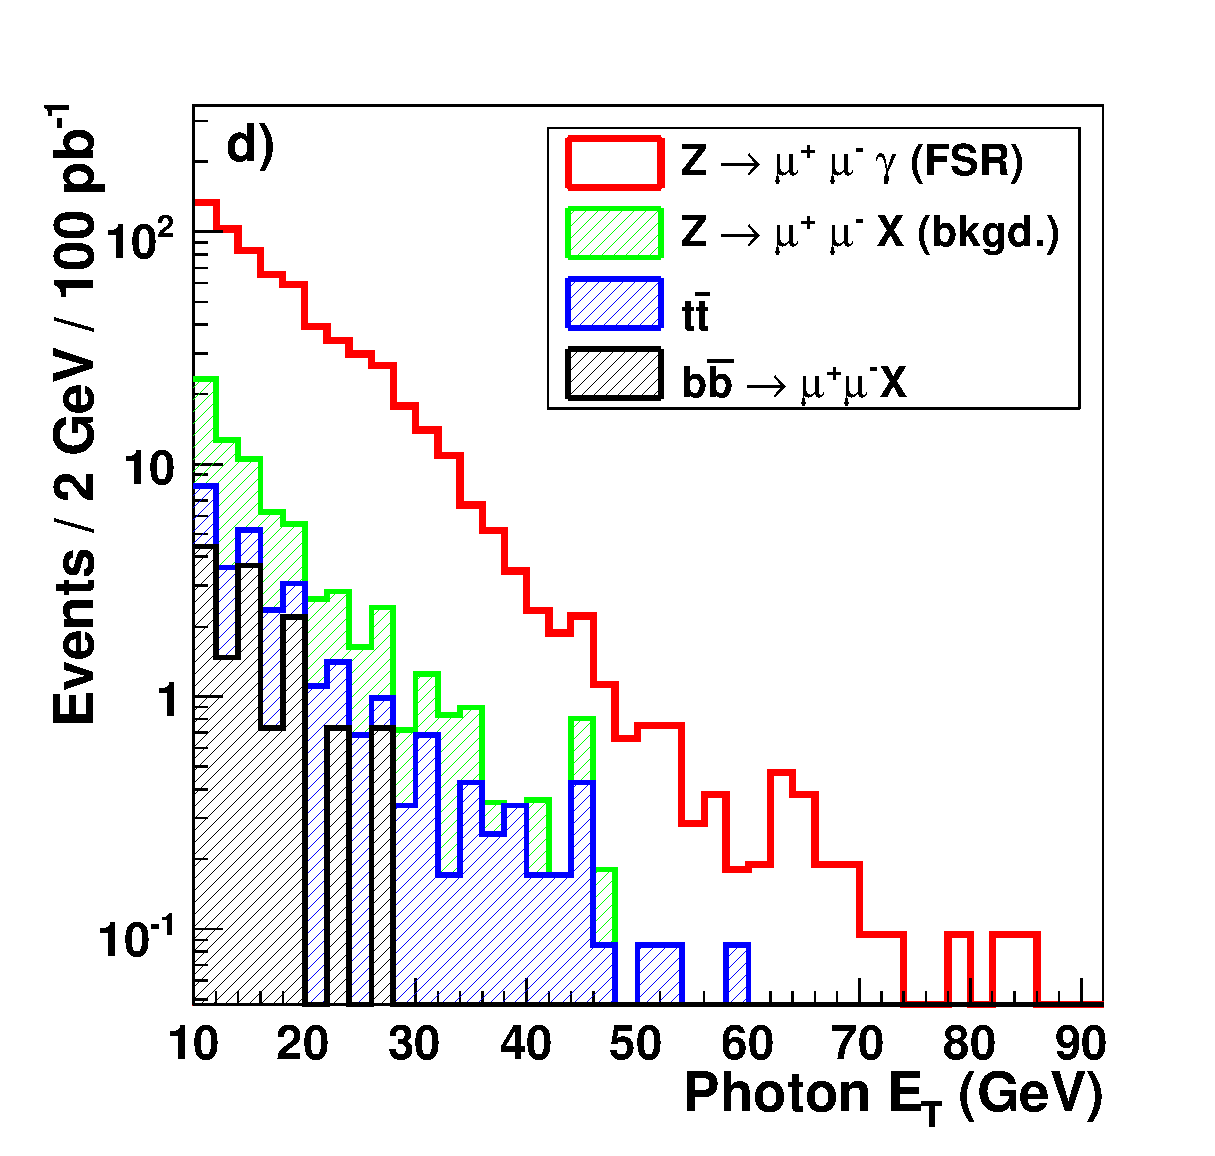
\includegraphics[width=0.46\linewidth]{zgammafigs/etG.eps} %%\\[2mm]
    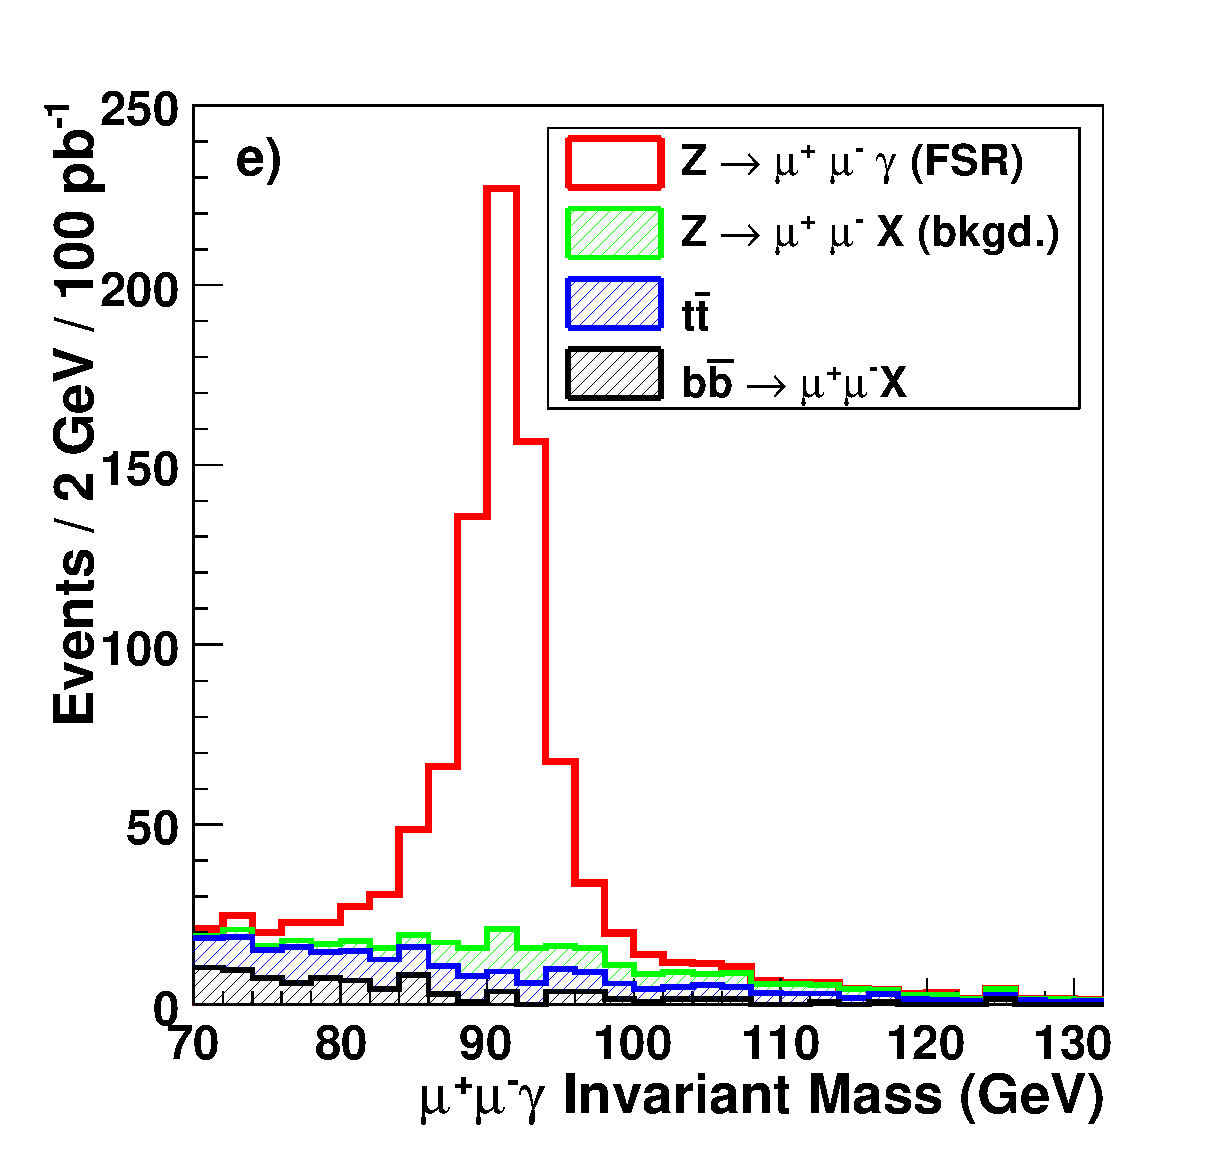
\includegraphics[width=0.46\linewidth]{zgammafigs/mMMG.eps}
    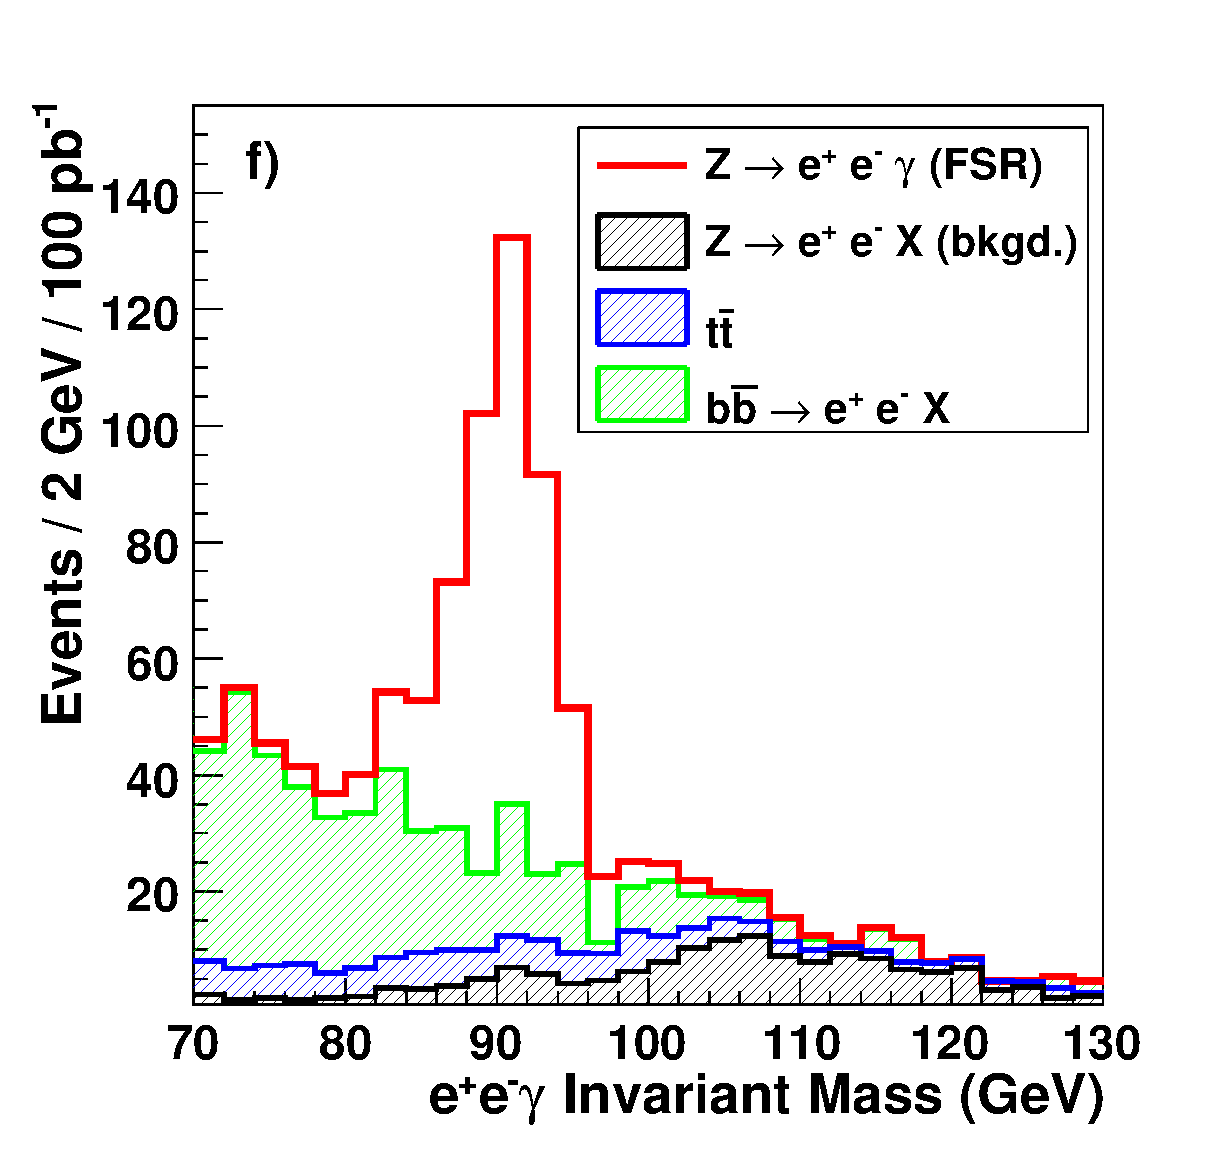
\includegraphics[width=0.46\linewidth]{zgammafigs/meeg.eps} %%\\[2mm]
\caption{
``N-1'' Distributions of a) $\Delta R$ distance between the closest muon and photon, 
b) invariant mass of the $\mu^+\mu^-$ system, and c) $E_T$ of the second leading central
jets, where all other cuts have been applied. The corresponding cut value is indicated
by an arrow. d) The $E_T$ spectrum of the photon candidates. Reconstructed $\ell^+\ell^- \gamma$ invariant 
mass for the obtained e) $\mu^+\mu^-\gamma$ and d) $\mathrm{e}^+\mathrm{e}^-\gamma$ samples.
}
%\vspace*{-0.3cm}
  \end{center}
\end{figure} \label{fig:llgamma}




In conclusion, the  $\mathrm{Z}\to \ell^+\ell^- \gamma$  process is expected to provide a clean sample
of about 1000 photons after 100~pb$^{-1}$. As neither calorimeter nor track isolation cuts on the
photon candidate have to be used in the event selection, this sample will provide us with an important
cross check of the photon ID studies performed with electrons. In particular, it will be useful
for studying effects of the photon conversions and track veto.

\section{Photon Fake Rates and Purity}
\subsection{Photon-Jet Fake Rate}
\subsection{Photon-Electron Fake Rate}


\section{Additional Backgrounds to Photons}
As previously mentioned, since photons only manifest themselves as isolated clusters of energy in the electromagnetic calorimeter, they are subject to backgrounds from cosmic ray and beam halo muons which undergo bremsstrahlung in the calorimeter as they pass through.  For each of these backgrounds, one attempts to derive the contamination from these sources by identifying variables that are sensitive to the difference between these bremsstrahlung backgrounds and building templates from the data using tags.  Then along with templates from prompt electromagnetic objects in data, one can do fits to the final candidate distributions in the data to determine the final prompt fraction.

The handles that we consider are:
\begin{itemize}
\item reconstructed time in the ECAL
\item shape of the ECAL energy deposition
\item reconstructing matching (in space and time) signals in HCAL and Muon systems   
\end{itemize}

\subsection{Beam Halo Muons}

%original text from Tia, edited by A.A.
"Halo muons" are a muons that travel along with the proton beams. They are
produced by beam protons hitting residual gas (or the sides of the
beam pipe), then showering to pions, which subsequent decay to muons.
These muons could leave evidence in the CMS detector through interacting with
the material.

There is halo shielding prior to the CMS detector, and there are halo
triggers to reject halo events (or select them for the purposes of alignment). 
Some muons may still leave evidence in the recorded events.  If a muon crosses through the 
ECAL and bremsstrahlungs, this process could be mistaken for a prompt photon. 
We are currently investigating the shower shape and timing of a halo muon bremsstrahlung compared with
the shower shape and timing of prompt photons.  It is expected that halo muon
bremsstrahlung shower shape will be extended in eta (halo muons travel
parallel to beam), while the prompt photon shower shape will be well constrained, if perhaps
extended in phi (if the photon converts to an e- e+ pair, the strong
magnetic field will bend the pair to extend its energy deposit in phi).
\subsubsection{ECAL timing}

\subsubsection{shower shape}

\subsubsection{ECAL-CSC correlations}

\subsubsection{ECAL-HE correlations}
For beam halo Monte Carlo events, a correlation is observed between depositions of energy in the
HCAL Endcap (HE) and the ECAL barrel.  If the difference in phi between these deposits is constructed
(for a significant amount of energy in the HE), one can see an obvious peak (see Figure~\ref{fig:BHdPhi}).

Using this correlation, one may `tag' photon events as originating from beam halo.  For a given
reco::Photon to be identified as beam halo in this way:
\begin{list}{$\bullet$}
\item{The difference between the EB photon position and the HE energy deposition must be smaller than
0.08 in $\Delta\phi$.}
\item{The energy of the HE rechit for satisfying the cut must be greater than XX GeV.}
\end{list}
In principle, the timing information for the HE may also be exploited to provide further evidence that
this photon originates from an out-of-time background.

`Tagging' these beam halo events has a dual purpose.  In the data, tagging these events with high
purity will allow for studies of the photons that originate from beam halo for the purposes of 
study and statistical separation.  At the same time, if the tag is of sufficient efficiency, one
may in turn use the tag to discriminate against potential signal candidate events which also show
this correlation.  In the data, this may be checked against prompt electromagnetic objects, such as 
W$\rightarrow e\nu$, wherein the number of events rejected by applying the tag can give a handle on
the efficiency of using this tag as a veto.

A Monte Carlo exercise was performed to determine an operating point for the tagger cuts listed above.  It
was found that XX\% of W$\rightarrow e\nu$ events were rejected by the veto, and a corresponding YY\%
of beam halo Monte Carlo (in which there was a supercluster of ZZ~GeV present) were accepted.

\subsection{Cosmic Ray Muons}

\subsubsection{shower shape}

\begin{figure}[hbtp]
  \begin{center}
    \resizebox{10cm}{10cm}{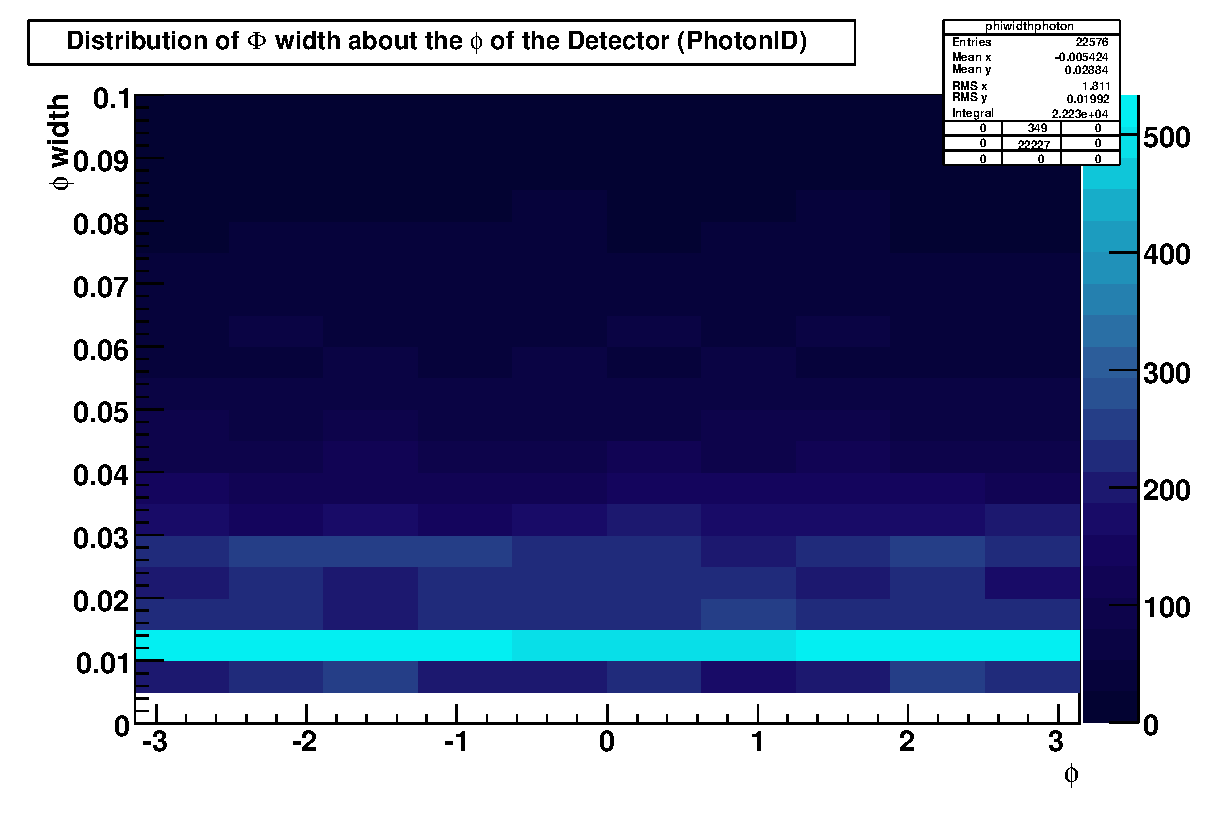
\includegraphics{CosmicPlots/photonID.eps}}
    \caption{The energy weighted width in $\phi$ as a function of detector $\phi$ for prompt, direct photons from the interaction region.  No dependence is observed.}
    \label{fig:PromptPhiWidPhi}
  \end{center}
\end{figure}

\begin{figure}[hbtp]
  \begin{center}
    \resizebox{10cm}{10cm}{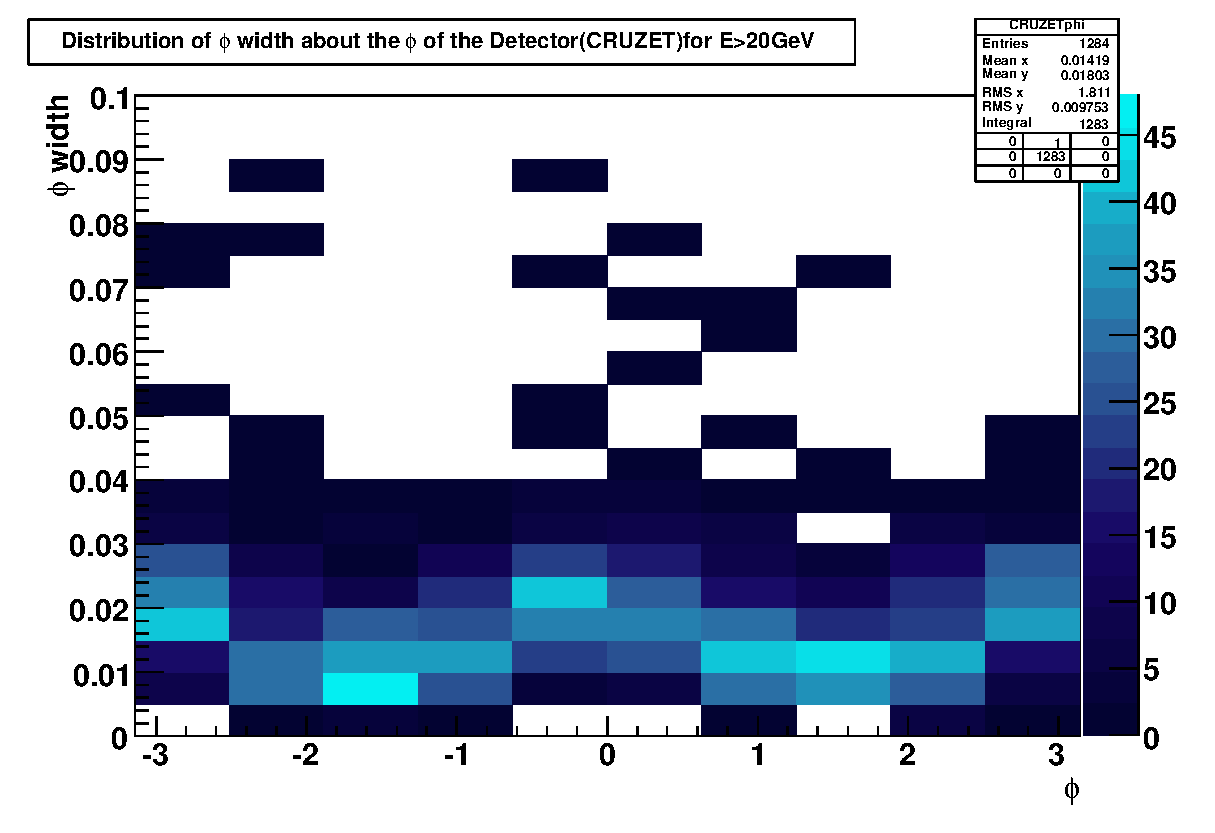
\includegraphics{CosmicPlots/CRUZET.eps}}
    \caption{The energy weighted width in $\phi$ as a function of detector $\phi$ for electromagnetic objects found in
CRUZET events.}
    \label{fig:CRUZETPhiWidPhi}
  \end{center}
\end{figure}

\subsubsection{ECAL - Muon Correlations}


\section{Summary}

\begin{thebibliography}{9}
\bibitem{uug_note}  Y. Gershtein, ``Preparing for Measurement of Photon Identification Efficiency and Energy Scale Using mu mu gamma Final State,'' CMS Note AN-2005/040. 
\bibitem{NancyConv}  N. Marinelli, ``Track finding and identification of converted photons.''  CMS Note 2006/005.


\end{thebibliography}
 
%------------------------------------------------------------------------------
\pagebreak
\appendix
\section{Photon Energy Scale}

\section{Photon Software Organization and Use}
\subsection{Infrastructure}
The software for the reconstruction and identification of photons is logically
divided into two parts to ensure flexibility.  


The first part, is encapsulated in the CVS package RecoEgamma/EgammaPhotonProducers.  
For each ECAL supercluster in the barrel or endcap which meets the 
preselection requirements, a reco::Photon object is created.  The preselection is based
on a combination of the supercluster transverse energy, the $HadOverEM$ ratio, and
isolation requirements.  At the time of this writing, only the requirement (10~GeV) on
the transverse energy is active.

The reco::Photon object is the reconstruction data format, and is designed to be as 
space efficient as possible. This object carries information about the original 
supercluster, the presence or absence of reconstructed conversions
\footnote{A separate, specific data format (reco::Conversion) is 
defined for conversions, which carries information about the reconstructed track(s), 
fitted vertex, and associated clusters.  For more information about the conversion
finding, please see~\cite{NancyConv}}, 
and the presence of pixel hits (which could be an indication that the object is in 
reality an electron).  The photon candidate is attributed an energy and a momentum,
the latter of which is calculated using the primary vertex of the photon (at the time
of this writing, the vertex from pixel triplets is used).  The energy assigned to the
photon is the energy in a 5x5 array of crystals if the previously defined R9 (see 
Eqn.~\ref{eqn:R9}) is greater than 0.93.  Otherwise, the energy is the same as the
supercluster energy.

The second part of the software infrastructure is the
CVS package RecoEgamma/PhotonIdentification.  For every reco::Photon object that 
is created, a corresponding reco::PhotonID object is created, and an association 
made and stored in the Event.  The purpose of the ``helper'' object reco::PhotonID is to 
provide additional information in order to allow users to select reconstructed photon 
objects that satisfy at least the criteria set forth in this note.  The reco::PhotonID 
object (stored in DataFormats/EgammaCandidates) contains information on the isolation of 
the photon (calculated using the RecoEgamma/EgammaIsolationAlgos) as well as several
flags concerning the position of the photon with respect to both the barrel-endcap junction and the 
supermodule boundaries and fiducial locations in detector $\eta-\phi$.  Quality flags, 
defined for {\bf LooseEM}, {\bf LoosePhoton} and {\bf TightPhoton} are also set based 
on the criteria defined in the configuration file.

\subsection{Photon Isolation}
Tools to compute various isolation variables for electrons and photons are available in the
package RecoEgamma/EgammaIsolationAlgos.  These are the tools called by RecoEgamma/PhotonIdentification 
for the calculation of the isolation.

For verion 2\_1\_0 of the CMSSW software this package has been extensively reworked, to produce 
reco::IsoDeposit. These ``Isodeposits'' store the basic information about each of the objects 
isolated against (crystals in the ECAL, tracks, etc.) and thus allow the the isolation to be 
recomputed with varying cuts on cone size, $E_T$ thresholds and similar variables, even if the 
original objects have been dropped.  Compared to the previous implementation, this switch 
provides increased flexibility. Additionally, the improved isolation code is structurally parallel 
to the muon isolation code, easing the implementation of higher level analysis.
The approach has been been tested and shown to work well for HCAL and track isolation.
For the ECAL-isolation, physics performance has been shown to be good, but technical issues 
remain to be adressed.  In particular the large number of crystals contained in typical isolation 
cones leads to large disk-space requirements and long execution times. Several solutions 
are currently under study.

\section{Photon Identification at High Energies}

\end{document}
